% Created 2025-04-11 ven. 11:33
% Intended LaTeX compiler: pdflatex
\documentclass[11pt]{article}
\usepackage[utf8]{inputenc}
\usepackage[T1]{fontenc}
\usepackage{graphicx}
\usepackage{longtable}
\usepackage{wrapfig}
\usepackage{rotating}
\usepackage[normalem]{ulem}
\usepackage{amsmath}
\usepackage{amssymb}
\usepackage{capt-of}
\usepackage{hyperref}
\usepackage{listings}
\usepackage{lmodern} % Ensures we have the right font
\usepackage{graphicx}
\usepackage{amsmath, amsthm, amssymb}
\usepackage[table, xcdraw]{xcolor}
\usepackage{fancyhdr}
\usepackage[lined,boxed,commentsnumbered,ruled,vlined,linesnumbered]{algorithm2e}
\SetKwComment{Comment}{$\triangleright$\ }{}
\usepackage[left=2cm,right=2cm,top=3cm,bottom=3cm]{geometry}
\pagestyle{fancy}
\makeatletter
\edef\mytitle{\@title}
\makeatother
\fancyhead{} % clear all fields
\fancyhead[L]{\slshape \rightmark}
\renewcommand{\headrulewidth}{0.1pt}
\fancyfoot{} % clear all fields
\fancyfoot[R]{Page \thepage}
\renewcommand{\footrulewidth}{0pt}
\usepackage{titling}
\setlength{\droptitle}{-8ex}
\pretitle{\begin{flushleft}\Large\bfseries}
\posttitle{\par\end{flushleft}}
\preauthor{\begin{flushleft}\large}
\postauthor{\end{flushleft}}
\predate{\begin{flushleft}}
\postdate{\end{flushleft}}
\usepackage[normalem]{ulem}
\usepackage{sectsty}
\sectionfont{\underline}
\usepackage[font={color=gray},figurename=Fig.,labelfont={it}]{caption}
\usepackage{listings}
\usepackage{tikz}
\usepackage{lstautogobble}  % Fix relative indenting
\usepackage{color}          % Code coloring
\usepackage{zi4}            % Nice font

\definecolor{bluekeywords}{rgb}{0.13, 0.13, 1}
\definecolor{greencomments}{rgb}{0, 0.5, 0}
\definecolor{redstrings}{rgb}{0.9, 0, 0}
\definecolor{graynumbers}{rgb}{0.5, 0.5, 0.5}
\definecolor{grayW}{rgb}{0.96,0.96,0.97}

\usepackage{listings}
\lstset{
backgroundcolor=\color{grayW},
autogobble,
columns=fullflexible,
showspaces=false,
showtabs=false,
breaklines=true,
showstringspaces=false,
breakatwhitespace=true,
escapeinside={(*@}{@*)},
commentstyle=\color{greencomments},
keywordstyle=\color{bluekeywords},
stringstyle=\color{redstrings},
numberstyle=\color{graynumbers},
basicstyle=\ttfamily\footnotesize,
frame=tlbr,
framesep=12pt,
xleftmargin=12pt,
tabsize=4,
captionpos=b,
framexleftmargin=15pt,
framerule=0pt
}
\setlength{\arrayrulewidth}{0.3mm}
\setlength{\tabcolsep}{3pt}
\renewcommand{\arraystretch}{1.2}
\usepackage[skip=0pt, parfill]{parskip}
\usepackage{tocloft}
\renewcommand{\cftsecleader}{\cftdotfill{\cftdotsep}}
\setlength{\parindent}{0pt}
\usepackage[fontsize=10pt]{fontsize}
\usepackage{setspace}
\setstretch{1,25}
\usepackage{forest}
\usepackage[linesnumbered]{algorithm2e}
\usepackage{tikz}
\setlength{\parindent}{0pt}
\author{Author: Enzo Durel \newline Professor: Dr. Chongle Pan}
\date{\today}
\title{CS5473 - Project 5}
\hypersetup{
 pdfauthor={Author: Enzo Durel \newline Professor: Dr. Chongle Pan},
 pdftitle={CS5473 - Project 5},
 pdfkeywords={},
 pdfsubject={},
 pdfcreator={Emacs 30.1 (Org mode 9.7.11)}, 
 pdflang={English}}
\begin{document}

\maketitle
\begin{center}
\includegraphics[width=10cm]{/home/hozen/orgmode_latex_export_img/ou_logo.png}
\end{center}
\thispagestyle{empty}
\setcounter{tocdepth}{2}
\tableofcontents
\clearpage
\pagenumbering{arabic}
\thispagestyle{empty}
\listoftables
\clearpage
\pagenumbering{arabic} 
\newpage
\section{Problem 1}
\label{sec:orgc1cffa7}

\subsection{Runtimes}
\label{sec:orgdb87da5}

\begin{table}[htbp]
\caption{Problem 1 Runtime}
\centering
\begin{tabular}{|l|c|c|c||c|}
\hline
Integers & 1M & 2M & 4M & 8M\\
\hline
Same RT & 0.0002394965 & 0.0004862981 & 0.0012506239 & 0.0032828204\\
\hline
Diff RT & 0.0004300362 & 0.0008670914 & 0.0017082404 & 0.0039351337\\
\hline
\end{tabular}
\end{table}
\subsection{Same Node}
\label{sec:orga34ba45}

\begin{itemize}
\item Latency \(\approx -3.488867e-04 s\)
\item Bandwidth \(\approx 9016.07 MB/s\)
\end{itemize}
\subsection{Diff Node}
\label{sec:orgd9fb1bd}

\begin{itemize}
\item Latency \(\approx -1.498357e-04 s\)
\item Bandwidth \(\approx 7957.72 MB/s\)
\end{itemize}
\subsection{Linear Regression}
\label{sec:org58f3f67}

\begin{center}
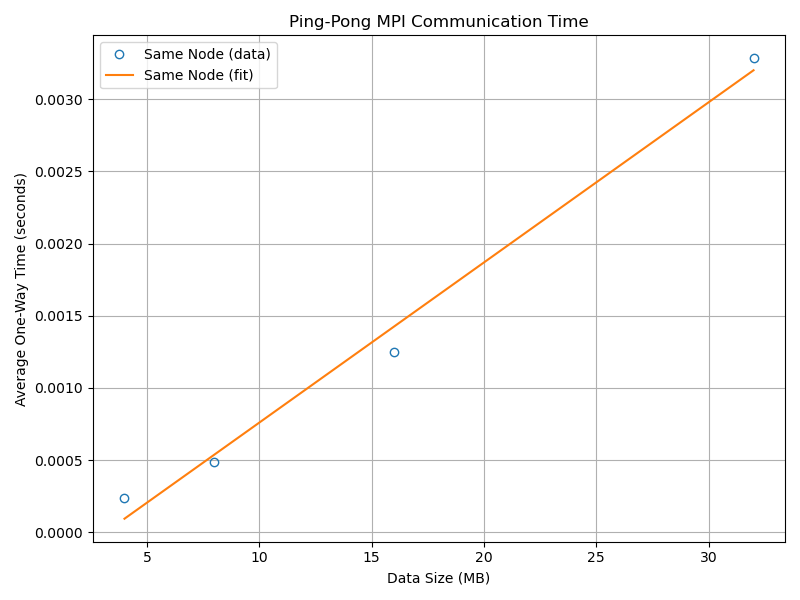
\includegraphics[width=10cm]{./img/pingpong_same_plot.png}
\captionof{figure}{Linear Regression for same}
\end{center}

\begin{center}
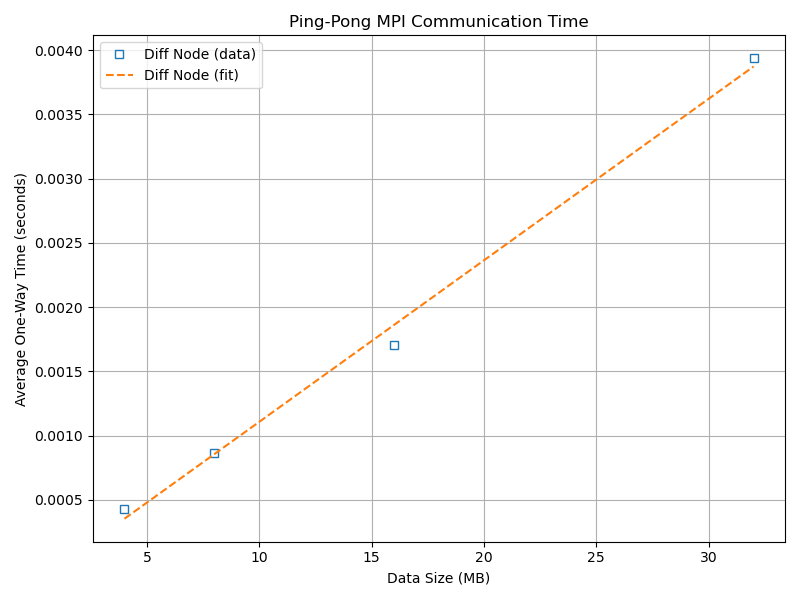
\includegraphics[width=10cm]{./img/pingpong_diff_plot.png}
\captionof{figure}{Linear Regression for diff}
\end{center}

\begin{center}
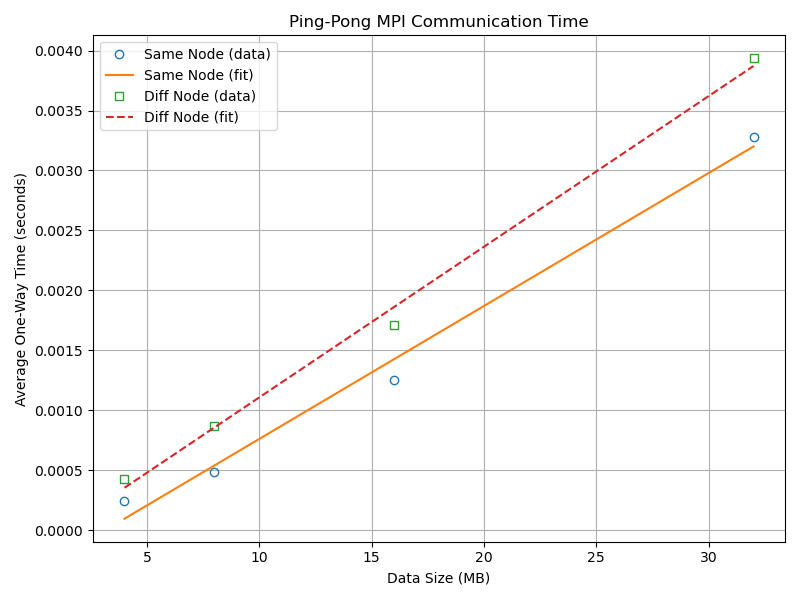
\includegraphics[width=10cm]{./img/pingpong_communication_plot.png}
\captionof{figure}{Linear Regression for both methods}
\end{center}
\end{document}
